\documentclass[oneside,senior,etd]{BYUPhys}

\usepackage{cmap} % Для корректной кодировки в pdf
\usepackage[utf8]{inputenc}
\usepackage{rotating}

\usepackage[russian]{babel}
\usepackage{amsfonts} % Пакеты для математических символов и теорем
\usepackage{amstext}
\usepackage{amssymb}
\usepackage{amsthm}
\usepackage{graphicx} % Пакеты для вставки графики
\usepackage{subfig}
\usepackage{color}
\usepackage[unicode]{hyperref}
\usepackage[nottoc]{tocbibind} % Для того, чтобы список литературы отображался в оглавлении
\usepackage{verbatim} % Для вставок заранее подготовленного текста в режиме as-is
\usepackage{listings}

\newcommand{\sectionbreak}{\clearpage} % Раздел с новой станицы

\usepackage{tikz}
\usepackage{pgfplots}
\usetikzlibrary{arrows,positioning}
\usepackage{adjustbox}

\usepackage{makecell}
\usepackage{booktabs}
\usepackage{boldline}

\usepackage{xcolor}
\usepackage{soul}
\usepackage{url}
\usepackage{multirow}
\usepackage{amsmath}

\usepackage{pifont}
\usepackage{indentfirst} % Делать отступ в начале первого параграфа

% Общие параметры листингов
\lstset{
  %frame=TB,
  showstringspaces=false,
  tabsize=4,
  basicstyle=\linespread{1.0}\tt\small, % делаем листинги компактнее
  breaklines=true,
  texcl=true, % русские буквы в комментах
  captionpos=b,
  aboveskip=\baselineskip,
  commentstyle=\tt
}

\newcommand{\todo}[1]{\textcolor{red}{#1}}

% DEBUG
% \usepackage{showframe}

\Faculty{Факультет вычислительной математики и кибернетики}
\Chair{Кафедра системного программирования}
% Лаборатория
% \Lab{~}
\Year{2022}
  \Month{Май}
  \City{Москва}
  \AuthorText{Автор:}
  \Author{Доледенок Максим Вадимович}
  \AuthorEng{Max Doledenok}
  \AcadGroup{328}

  \TitleTop{Инструмент динамического анализа корректности раскладки}
  % Раскомментируйте, если нужны еще строчки названия
  \TitleMiddle{памяти в ОСРВ с поддержкой ARINC 653}
  % \TitleBottom{Третья строка названия}
  % Uncomment if you need English title
  % \TitleTopEng{Thesis theme, first line}
  % \TitleMiddleEng{Thesis theme, second line}
  % \TitleBottomEng{Thesis theme, third line}

\docname{Курсовая работа}
  \Advisor{Хорошилов Алексей Владимирович}
  \AdvisorDegree{к.ф.-м.н.\\}
  % Раскомментируйте, чтобы добавить научного консультанта
  \Consultant{Чепцов Виталий Юрьевич}
  %\ConsultantDegree{степень, звание\\}

% Закомментируйте, если аннотация не нужна
%\Abstract{
%Аннотация.
%}
% Раскомментируйте, если нужна английская аннотация
% \AbstractEng{Abstract in English}

% Раскомментируйте, чтобы написать благодарности
% \Acknowledgments{Благодарности.}

%%%% DON'T change this. It is here because .sty does not support cyrillic cp properly %%%%
\TitlePageText{Титульная страница}
\University{Московский государственный университет имени М.В.Ломоносова}
\GrText{гр.}
\AdvisorText{Научный руководитель}
\ConsultantText{Научный консультант}
\AbstractText{Аннотация}
\AcknowledgmentsText{Благодарности}
\ListingText{Листинг}
\AlgorithmText{Алгоритм}

% Set PDF title and author
\hypersetup{
  pdftitle={Курсовая},
  pdfauthor={Доледенок Максим}
}

\begin{document}
\fixmargins
 \makepreliminarypages

\oneandhalfspace

\newenvironment{compactlist}{
  \begin{list}{{$\bullet$}}{
  \setlength\partopsep{0pt}
  \setlength\parskip{0pt}
  \setlength\parsep{10pt}
  \setlength\topsep{8pt}
  \setlength\itemsep{0pt}
  }
  }{
  \end{list}
}

\pdfbookmark[section]{\contentsname}{toc}
\tableofcontents

\section{Введение}

\subsection{ОСРВ}

Операционные системы реального времени (ОСРВ) -- это операционные системы, одним из важнейших
требований к которым является выполнение поставленных задач за заранее определенное время.
Это отличает их от известных пользовательских операционных систем, где фактор времени не так
важен. ОСРВ используются там, где небольшая временная задержка может привести к существенным
проблемам. Например, в авиакосмической отрасли, на некоторых производствах, в системах
аварийной защиты.

\subsection{ОСРВ JetOS}

В данной курсовой работе рассматривается операционная система реального времени JetOS, разрабатываемая
в Институте Системного Программирования Российской Академии Наук. ОСРВ JetOS предназначена для
использования в авионике, в частности, в гражданских самолетах и спутниках. JetOS разрабатывается
в соответствии со стандартом ARINC 653, который регламентирует временное и пространственное
разделение ресурсов авиационной ЭВМ и определяет программный интерфейс, которым должно
пользоваться прикладное ПО для доступа к ресурсам ЭВМ. Единицей планирования ресурсов является
раздел, аналог пользовательской программы. Каждый раздел получает как процессорное время, 
так и некоторую часть оперативной памяти.

\subsection{Статическая конфигурация памяти}

В JetOS конфигурация памяти является статической, то есть раскладка памяти происходит
на этапе загрузки операционной системы, исходя из заранее описанной пользователем
конфигурации. При динамической конфигурации памяти пользовательские приложения могут
заимствовать области оперативной памяти для временного использования. Но для ОСРВ
это не всегда подходит, потому что сложно обеспечить детерминированность при работе
с памятью. А для ОСРВ JetOS детерминированность является очень важным фактором,
повышающим безопасность и отказоустойчивость операционной системы. Поэтому в JetOS
применяется строго статическая конфигурация памяти.

\subsection{Тестирование раскладки памяти}

Поскольку в ОСРВ JetOS требования к безопасности строгие, необходимо проверять,
что раскладка памяти происходит корректно. Из-за того что в раскладке памяти много
этапов, проверять каждый из них было бы сложно. Поэтому разумным представляется вариант
тестирования в динамике, то есть тестирование должно происходить во время исполнения
программы операционной системой. Тогда условия тестирования будут максимально близки
к реальным условиям использования ОСРВ.

\section{Постановка задачи}

Целью данной курсовой работы является разработка и интеграция в систему тестирования
инструмента для тестирования раскладки памяти в ОСРВ JetOS.

Для достижения цели курсовой работы нужно решить следующие задачи:
\begin{itemize}
  \item Необходимо изучить структуру раскладки памяти в ОСРВ JetOS.
  \item Придумать схему динамического тестирования раскладки памяти.
  \item Реализовать тестирование памяти разделов.
  \item Реализовать тестирование памяти ядра ОС.
  \item Реализовать быстрый алгоритм тестирования, который тестирует память выборочно.
  \item Интегрировать тесты в систему тестирования.
\end{itemize}

\section{Обзор существующих решений}

Подобных инструментов в других ОС найти не удалось. Есть общеизвестные инструменты
динамического тестирования памяти, например Address Sanitizer. Это инструмент,
который обнаруживает различные ошибки по работе с памятью. Он обнаруживает
переполнение буфера, использование памяти после её обвобождения, обращения по невалидному адресу
и прочие. Но Address Sanitizer не подходит, потому что он проверяет корректность работы с памятью
самой программы, а не устройство раскладки памяти.

В самой ОСРВ JetOS есть встроенная проверка раскладчика памяти, но она проверяет
конфигурацию памяти статически, без запуска проекта. И проверяется только корректная
работа раскладчика. А ошибки могут происходить и на стадии загрузки ОС. Из-за этого
невозможно быть полностью уверенным в корректной раскладке памяти. Например, права
доступа к памяти при раскладке могут назначаться одни, а в реальности,
в результате неправильной работы загрузчика, могут оказаться другими.

\section{Исследование и простроение решения задачи}

\subsection{Устройство памяти в ОСРВ JetOS}

Основные принципы устройства памяти в ОСРВ JetOS:
\begin{itemize}
  \item платформа имеет одно или несколько ядер процессора;
  \item набор регионов физической памяти общий для всех ядер;
  \item на одной платформе может быть запущено несколько модулей,
  здесь модуль -- сконфигурированная операционная система, предназначенная для выполнения
  на одном или нескольких ядрах процессора на платформе;
  \item память разделяется на виртуальную и физическую;
  \item виртуальная память своя для каждого модуля, физическая -- общая для всех модулей;
  \item виртуальная память разделяется на привилегированную (доступную только ядру)
  и непривилегированную (доступную и ядру, и разделам);
  \item физическая память разделяется на оперативную память и память физических устройств;
  \item и виртуальная, и физическая память делятся на страницы;
  \item размеры страниц одинаковы для виртуальной и физической памяти;
  \item адрес страницы пропорционален ее размеру.
\end{itemize}

\subsection{Блоки памяти}

В результате работы раскладчика в виртуальной памяти выделяются блоки памяти.
Блок памяти — это непрерывная область виртуальной памяти.
Каждый раздел обладает своими блоками памяти, к которым нет доступа у других разделов
(если этот блок не является разделяемым). Также у каждого модуля есть свои блоки памяти ядра,
к которым нет доступа из разделов и из других модулей.

Блок памяти обладает следующими атрибутами:
\begin{itemize}
  \item виртуальный адрес блока памяти;
  \item физический адрес блока памяти;
  \item размер блока памяти;
  \item коэффициент выравнивания;
  \item политика кэширования;
  \item права доступа: на чтение, на запись, на исполнение;
  \item наличие зоны безопасности перед блоком и/или после блока;
  \item размер зон безопасности перед блоком и/или после блока;
  \item флаг непрерывности блока в физической памяти;
  \item характер блока памяти: является ли он блоком оперативной памяти или блоком памяти
  физических устройств;
  \item список непрерывных отображений виртуальных адресов блока памяти на физические адреса;
  \item некоторые другие атрибуты.
\end{itemize}

Ещё блок памяти может быть разделяемым. Это значит, что он доступен
сразу нескольким разделам. Каждый раздел имеет доступ к такому блоку
с правами доступа, описанными для каждого раздела. Причем разделы
могут быть при этом в разных модулях.

Виртуальная память между блоками памяти может иметь либо права доступа одного из двух
соседних блоков памяти, либо объединение прав доступа соседних блоков, либо вообще
не иметь прав доступа ни на чтение, ни на запись, ни на исполнение.

\subsection{Требования к тестированию}

Тестирование в основном заключается в проверке прав доступа разделов или ядра к некоторым адресам
виртуальной памяти.

Для каждого раздела нужно тестировать права доступа к:
\begin{itemize}
  \item своим блокам памяти;
  \item блокам памяти ядра;
  \item зонам безопасности до/после блоков памяти;
  \item памяти между блоками;
  \item разделяемым блокам памяти.
\end{itemize}

Для ядра нужно тестировать права доступа к:
\begin{itemize}
  \item своим блокам памяти;
  \item блокам памяти разделов;
  \item зонам безопасности до/после блоков памяти;
  \item памяти между блоками.
\end{itemize}

Также надо тестировать разделяемые блоки памяти. То есть проверять, что если раздел
записал данные в разделяемый блок, то другой раздел может эти данные считать.

\subsection{Основные принципы тестирования раскладки памяти}

\subsubsection{Конфигурация}

Программа для тестировния не может находиться в разделе, потому что у раздела
ограниченные возможности. Например, из раздела нельзя будет посмотреть файлы
конфигурации памяти, которые формирует раскладчик.
Значит, инструмент для тестирования должен находиться вне JetOS. Инструмент для 
тестирования называется memtest, и представляет собой программу на языке Python. 
Python был выбран из-за того, что система сборки JetOS написана на Python, а также
там есть нужные классы для блоков памяти, разделяемых блоков и чтения файлов формата
yaml. Именно в этом формате хранятся файлы конфигурации памяти.

Общение с разделами происходит через UART. Для этого в JetOS есть такая абстракция,
как потоки, каждый из которых связывается с TCP-портом, к которому может подключиться memtest.
Из TCP-порта данные отправляются в UART, из которого уже их читает JetOS.
Для каждого модуля выделяются свои потоки. Основными являются потоки USR и KRN,
через USR поток осуществляется ввод/вывод для разделов, а через KRN поток -- ввод/вывод
для ядра. USR поток является общим для всех разделов.

Чтобы условия тестирования были максимально приближены к реальным, чтение, запись или исполнение
памяти осуществляется разделом при тестировании раздела, и ядром при тестировании ядра.
Причем если в проекте несколько разделов, нужно тестировать память каждого. Для этого
в JetOS была реализована библиотека, которая при тестировании автоматически
подключается к разделу и начинает ждать сообщений от memtest. То есть осуществляет
чтение в бесконечном цикле.

Поскольку USR поток общий для всех разделов в одном модуле, посылать через него сообщения
разным разделам было бы достаточно сложно. Поэтому для тестирования разных разделов
использовался механизм расписаний в JetOS. Расписание задаёт порядок и периодичность
выполнения разделов. При тестирования раскладки памяти для каждого раздела создаётся своё
расписание, в котором всё свободное время процессора выделяется ему. В итоге тестируется сначала
один раздел, потом переключается расписание, тестируется другой раздел, и так далее.

\subsubsection{Исполнение команд в JetOS при тестировании раздела}

Схему тестирования со стороны JetOS можно посмотреть на рис. \ref{testing_scheme}.
Разделу посылаются команды на чтение, запись или исполнение данных по определенному виртуальному адресу.
Раздел пытается выполнить эту команду. Если команда была выполнена успешно, раздел
отвечает инструменту. Иначе происходит прерывание, управление передаётся обработчику
прерываний. В нём обработчик передаёт управление обработчику прерываний раздела,
такой инструментарий есть в JetOS. Этот обработчик пишет в USR поток сообщение о прерывании
и перезапускает раздел. Далее раздел снова ждёт сообщений от инструмента.

\begin{figure}[t]
  \centering
  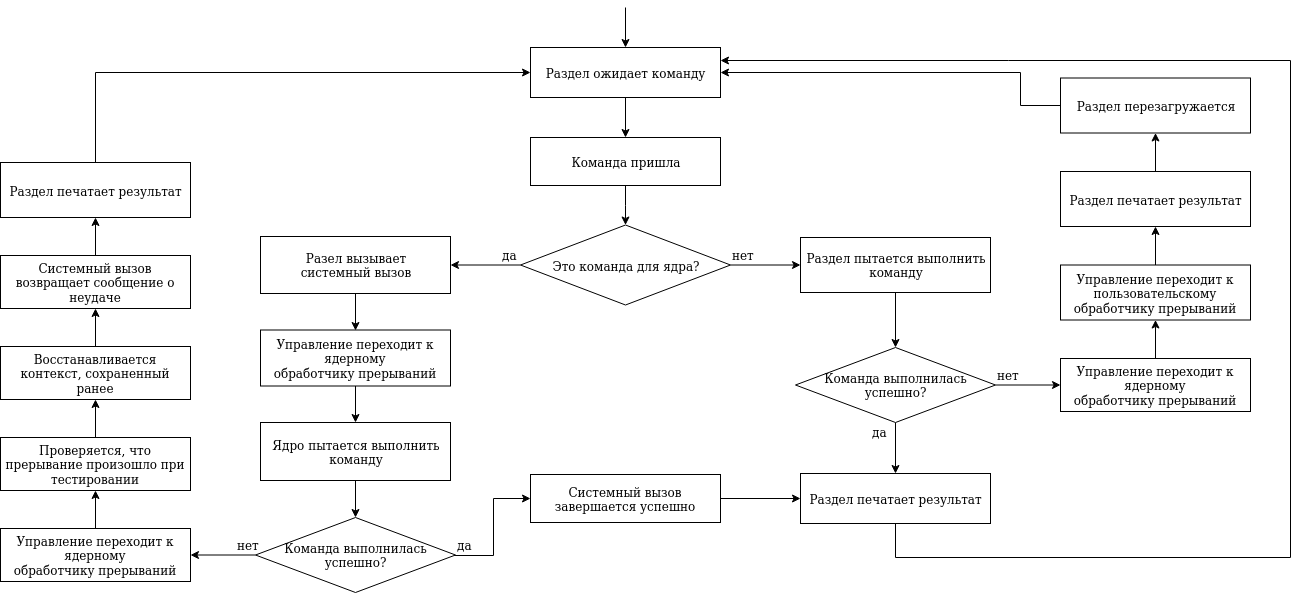
\includegraphics[width=\textwidth]{./testing_scheme.png}
  \caption{Схема тестирования со стороны JetOS}
  \label{testing_scheme}
\end{figure}

\subsubsection{Исполнение команд в JetOS при тестировании ядра}

Разделу посылаются команды на чтение, запись или исполнение данных по определенному виртуальному адресу.
Раздел вызывает системный вызов, в аргументах передавая адрес. Этот вызов поступает
обработчику системных вызовов, который находится в библиотеке, подключаемой к ядру
при тестировании раскладки памяти. В обработчике ядро сначала сохраняет текущий контекст,
потом пытается считать, записать или
исполнить память по определенному адресу. Если это удаётся, системный вызов завершается
успешно, управление возвращается разделу, и он пишет сообщение об успешно выполненной
команде. Иначе происходит прерывание, и в его обработчике проверяется, равен ли адрес,
при чтении/записи/исполнении которого возникло прерывание, адресу, который был передан
в системном вызове. И если равен, то восстанавливается контекст, сохранённый ранее, и 
системный вызов возвращает сообщение о неудаче. И раздел пишет сообщение о невыполненной
команде.


\subsection{Протокол взаимодействия memtest с разделом}

При запуске memtest посылает проверочное сообщение определённому разделу в определенном модуле, в
качестве конкретных чисел выбрано \dq\texttt{0x11 0x88 0xff 0x0}\dq.

Раздел посылает подтверждение вида \dq\texttt{0x11 0x88}\dq. После того, как инструмент получил подтверждение, 
он может посылать запросы разделу.

Запросы разделу посылаются в виде 4 или более шестнадцатиричных чисел:
\dq\texttt{<command> <address> <size> <data>}\dq, где

\begin{compactlist}
  \item \texttt{command} -- запрос на действие:
  \begin{itemize}
    \item 1 -- запрос на выполнение памяти из пользовательского режима;
    \item 2 -- запрос на запись в память из пользовательского режима;
    \item 3 -- запрос на запись с последующим чтением памяти из пользовательского режима;
    \item 4 -- запрос на чтение памяти из пользовательского режима;
    \item 5 -- запрос на переключение расписания модуля;
    \item 6 -- запрос на чтение ядерной памяти из ядра;
    \item 7 -- запрос на запись в ядерную память из ядра;
    \item 8 -- запрос на выполнение ядерной памяти из ядра;
    \item 9 -- запрос на чтение пользовательской памяти из ядра;
    \item 10 -- запрос на запись в пользовательскую память из ядра;
    \item 11 -- запрос на выполнение пользовательской памяти из ядра.
  \end{itemize}

  \item \texttt{address} -- адрес от 0 до \begin{math} 2^N \end{math} - 1, по которому хотим считать, записать или исполнить, где N -- размер слова;
  \item \texttt{size} -- размер считываемой или записываемой информации в байтах;
  \item \texttt{data} -- данные для записи в виде списка байт. Если был запрос на чтение или выполнение, передаётся \dq0\dq.

\end{compactlist}

Раздел посылает ответы, если удалось выполнить действие, в виде 2 или более шестнадцатичных чисел:
\dq\texttt{<command> <data>}\dq, где

\begin{itemize}
  \item \texttt{command} -- число от 1 до 11 -- сообщение об удачно выполненном запросе (возможные запросы описаны выше);
  \item \texttt{data} -- если был запрос на чтение, то передаются считанные данные побайтово.
  При запросе на запись передаётся информация, считанная из места, куда пытались записать.
\end{itemize}

Если произошло прерывании при попытке выполнить запрос, раздел отвечает \dq\texttt{0xff <address>}\dq,
где \texttt{address} -- адрес, по которому пытались считать, записать или выполнить. Либо выводится
сообщение о прерывании вида


\texttt{User code at 0x80001000 address tried to execute unmapped code at\\0x803e7000 address}


\subsection{Устройство инструмента memtest}

Сам инструмент -- это программа на языке Python.

Основные этапы его работы:
\begin{enumerate}
  \item Дождаться запуска JetOS.
  \item Сформировать нужные структуры для тестирования из файлов конфигурации, которые
  ранее создал раскладчик.
  \item Протестировать память ядра первого модуля.
  \item Отправить команду на переключение расписания, чтобы тестировать нужный раздел в модуле.
  \item Протестировать первый раздел первого модуля, вернуться к пункту 4, протестировать второй раздел и т.д.
  \item Протестировать разделяемую память первого модуля.
  \item Протестировать остальные модули аналогично пунктам 3-6.
  \item Протестировать разделяемую память, общую для нескольких модулей.
  \item Напечатать результаты тестирования.
\end{enumerate}

Само тестирование памяти для каждого раздела и для ядра происходит последовательно,
начиная с минимального виртуального адреса, и заканчивая максимальным. При этом,
тестировать каждый виртуальный адрес было бы слишком долго, поэтому тестируется
один виртуальный адрес из страницы.

\subsection{Алгоритм быстрого тестирования}

Но даже тестирование по одному виртуальному адресу из каждой страницы занимает достаточно
много времени. Поэтому был реализован алгоритм быстрого тестирования. Этот алгоритм
для каждой непрерывной области памяти с одинаковыми правами тестирует только 2 страницы.
Такими областями с одинаковыми правами являются например блок памяти или зона безопасности.
И если основной алгоритм тестирования может работать десятки часов, то быстрый алгоритм
работает чаще всего не больше минуты, при этом позволяя выявлять основные ошибки, допущенные
при раскладке памяти.

\subsection{Запуск тестирования}

Сейчас инструмент memtest внедрён в систему тестирования JetOS. Чтобы протестировать
какой-нибудь проект, нужно в его главной директории запустить команду

\texttt{\$ isp-test memtest=1}

И в случае положительного исхода тестирования, вывод будет как на рис. \ref{correct_test}.

\begin{figure}[t]
  \centering
  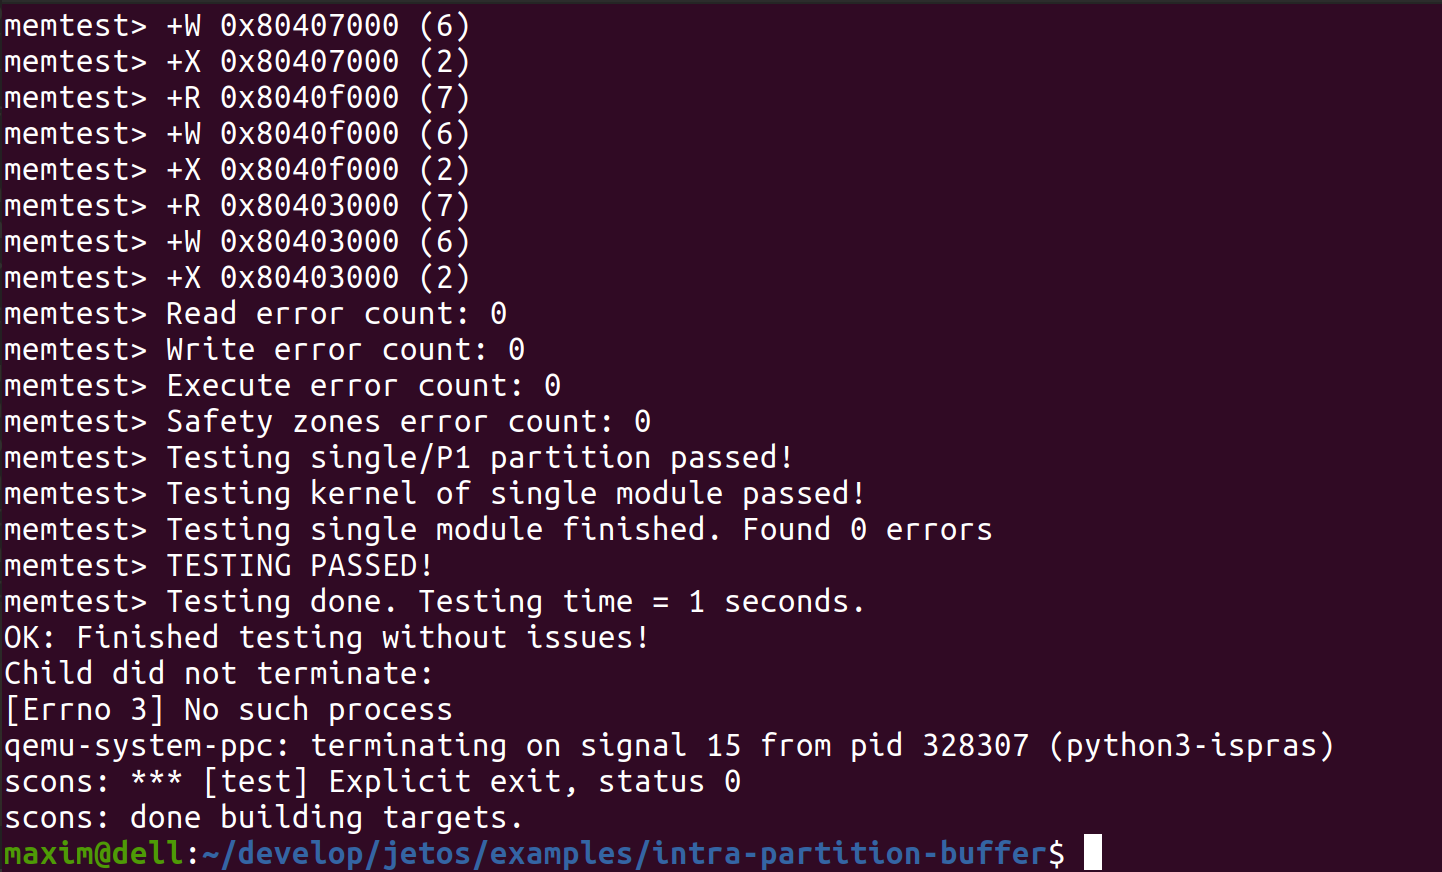
\includegraphics[width=0.9\textwidth]{./correct_test.png}
  \caption{пример трассы при завершении тестирования без ошибок}
  \label{correct_test}
\end{figure}

Если же на каком-то этапе тестирования произойдет ошибка, будет выдано сообщение
об ошибке как на рис. \ref{failed_test}.

\begin{figure}[t]
  \centering
  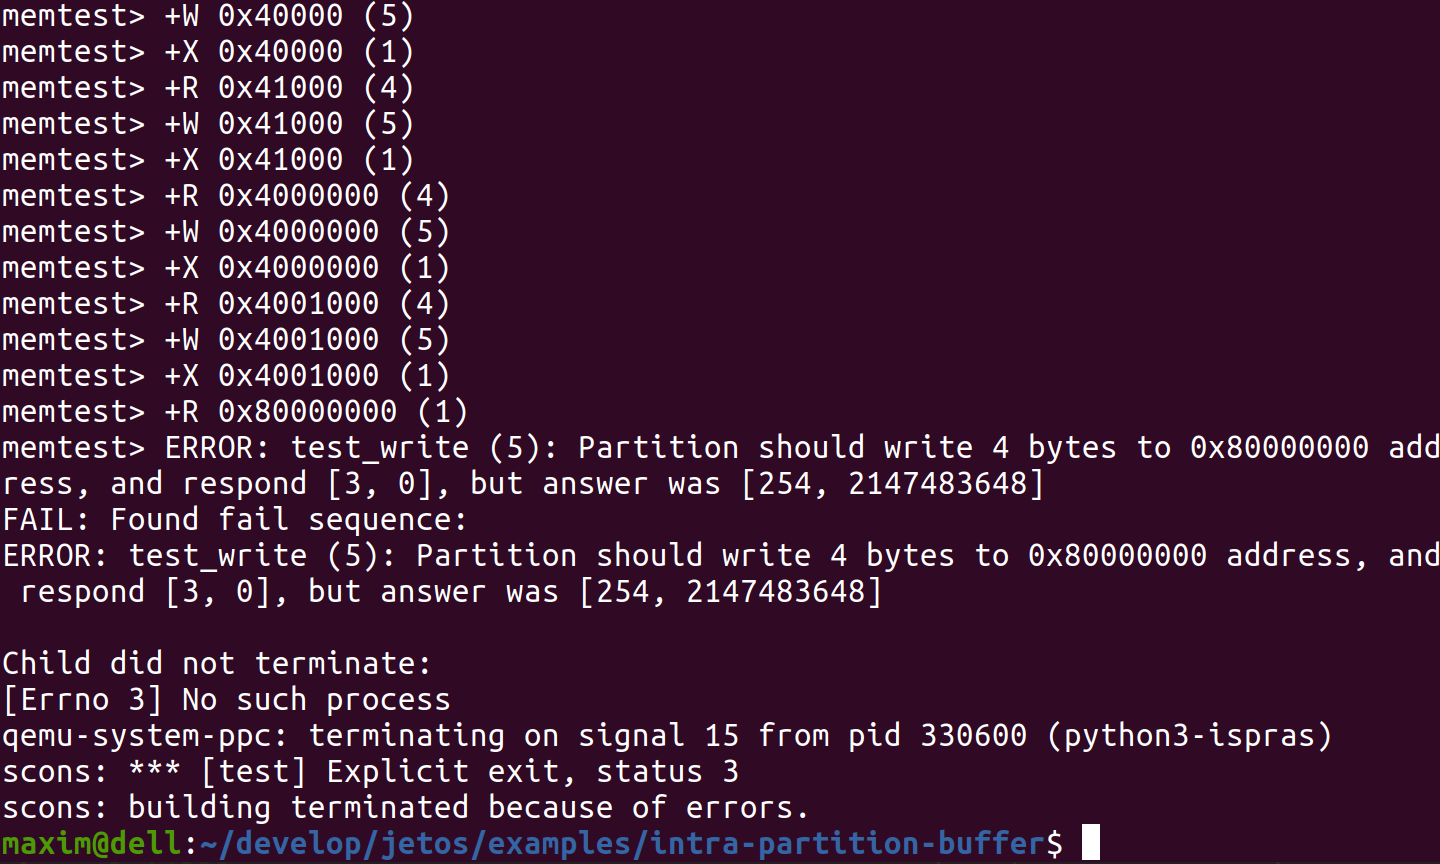
\includegraphics[width=0.9\textwidth]{./failed_test.png}
  \caption{пример трассы при завершении тестирования с ошибкой}
  \label{failed_test}
\end{figure}

\subsection{Результаты тестирования}

В результате быстрого тестирования на разных архитектурах были выявлены ошибки:

\begin{enumerate}
  \item На архитектуре MIPS раздел имел права доступа 'RWX' для блоков ядра.
  На уровне загрузчика не было никакой защиты ядерных блоков.
  \item На архитектуре PowerPC ядро могло читать данные из пользовательских блоков с правами
  только на чтение. Ошибка была на стадии создания конфигурации для раскладчика ОС.
  \item На архитектуре x86 раздел мог записывать данные в блок .ELF.0 с правами 'RX'.
  В раскладчике памяти были неверно указаны права доступа к пользовательской
  RO (только на чтение) памяти.
  \item При попытке чтения/записи ядром ОС в блок .LOADER\_SPIN на проектах, использующих одно ядро,
  возникало прерывание, хотя там права 'RW'. На самом деле, для проектов с одним ядром,
  этот блок памяти не должен выделяться совсем, но он выделялся на стадии загрузки ОС.
  \item На архитектуре PowerPC ядро могло исполненять данные в блоке памяти\\
  .LOADER\_FS, хотя там стоят права 'R'. Неверные права выставлялись в загрузчике.
\end{enumerate}

Также в процессе тестирования было найдено несколько ошибок, непосредственно
не связанных с ошибками при раскладке памяти. Все эти ошибки уже исправлены.

\section{Заключение}

В рамках курсовой работы была изучена работа раскладчика в ОСРВ JetOS, спроектирован
и реализован инструмент для тестирования раскладки памяти. Он был интегрирован в
систему тестирования, и сейчас быстрое тестирование используется в автоматических тестах
ОСРВ JetOS. В результате быстрого тестирования было найдено 5 ошибок раскладки памяти,
которые показывают, что реализация праактической части курсовой работает исправно.

\section{Дальнейшие планы}
\begin{itemize}

\item Написать для memtest особенные проекты для тестирования, в которых структура памяти
будет сложнее, чтобы более полно проверить корректность раскладки памяти.
Сейчас тестирование происходит на уже существующих проектах для JetOS.

\item При полном тестировании в зависимости от архитектуры можно существенно сократить количество
обращений к памяти из-за того, что память выделяется блоками фиксированного размера.
Также, поскольку полное тестирование памяти выполняется достаточно долго, можно
по ходу тестирования выдавать уверенность в корректном результате. Причем чтение из
разных адресов будет повышать эту уверенность по-разному, потому что виртуальный адрес,
по которому раскладчик выделил блок памяти, кратен размеру этого блока. Из-за этого
проверка корректности раскладки по адресам, имеющим б\'oльшую кратность размеру страницы,
в теории может отловить больше ошибок раскладчика, чем проверка по адресам, имеющим
меньшую кратность.

\item Сделать стратегию быстрого тестирования оптимальной, теоретически обосновать её оптимальность,
опираясь на выводы из предыдущего пункта.
\end{itemize}

\nocite{arinc, sanitizer, scons, jetos, allocator}

%\begingroup
\bibliographystyle{gost780u.bst}
\raggedright

\bibliography{references}
%\cite{arinc, scons, jetos, allocator}
%\endgroup


%\bibliographystyle{gost780u.bst} % Для соответствия требованиям об оформлении списка литературы
%\raggedright
%\bibliography{references}

% Раскомментируйте, если нужно приложение
% \appendix

% \cleardoublepage \phantomsection
% \section*{Приложение}
% \addcontentsline{toc}{section}{Приложение}

\end{document}
